\documentclass[12pt]{article}
\usepackage[utf8]{inputenc}
% PACKAGE FIGURE
\usepackage{caption}
\usepackage{graphicx}
% PACKAGE MARGE
\usepackage[top=2cm, bottom=2cm, left=2.5cm, right=2.5cm]{geometry}
% PACKAGE COULEUR
%\usepackage{color}
\usepackage{xcolor}
\usepackage{amsmath}
\usepackage[version=3]{mhchem} % Formula subscripts using \ce{}
% PACKAGE POUR LE WARNING
\newcommand\Warning{%
 \makebox[1.4em][c]{%
 \makebox[0pt][c]{\raisebox{.1em}{\small!}}%
 \makebox[0pt][c]{\color{red}\Large$\bigtriangleup$}}}%
% PACKAGE ENCADRE
\usepackage{calc}
\usepackage{tcolorbox}
\newtcolorbox{mybox1}[1]{colback=red!5!white,colframe=red!75!black,fonttitle=\bfseries,title=#1}
\newtcolorbox{mybox2}[1]{colback=blue!5!white,colframe=blue!75!black,fonttitle=\bfseries,title=#1}
\newtcolorbox{mybox3}[1]{colback=green!5!white,colframe=green!75!black,fonttitle=\bfseries,title=#1}
\newtcbox{\mybox}{nobeforeafter,colframe=black,colback=black!10!white,boxrule=0.5pt,arc=4pt,
  boxsep=0pt,left=6pt,right=6pt,top=6pt,bottom=6pt,tcbox raise base}
\newtcolorbox{mybox4}[1]{colback=white!5!white,colframe=white!75!black,fonttitle=\bfseries,title=#1}

\usepackage[sort&compress]{natbib}
\citestyle{nature}

% PACKAGE COLONNE
\usepackage{multirow}
% PACKAGE NUMEROTATION PAGE
\usepackage{fancyhdr}

\usepackage{hyperref}
\hypersetup{
    colorlinks=true,
    linkcolor=blue,
    filecolor=magenta,      
    urlcolor=cyan,
}

% DEBUT DU DOCUMENT
% PAGE DE PRESENTATION
\begin{document}
\begin{minipage}[c]{0.5\linewidth}

\includegraphics[scale=0.2]{latex_files/EPFL-logo.png}
\end{minipage}
\begin{minipage}[c]{0.5\linewidth}
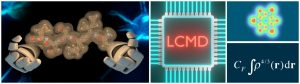
\includegraphics[scale=0.75]{latex_files/lcmd-logo.jpg}
\end{minipage}
\vspace{0.5cm}
\hrule 
\vspace{0.5cm}
\begin{center}
\LARGE \textbf{\textcolor{red}{M}olecular \textcolor{red}{D}ynamics meets \textcolor{red}{N}eural \textcolor{red}{N}etworks}: \\
\LARGE \textbf{TUTORIAL}
\vspace{0.5cm}
\\ % The assignment title
\end{center}
\hrule 
\vspace{2cm}
\begin{center}
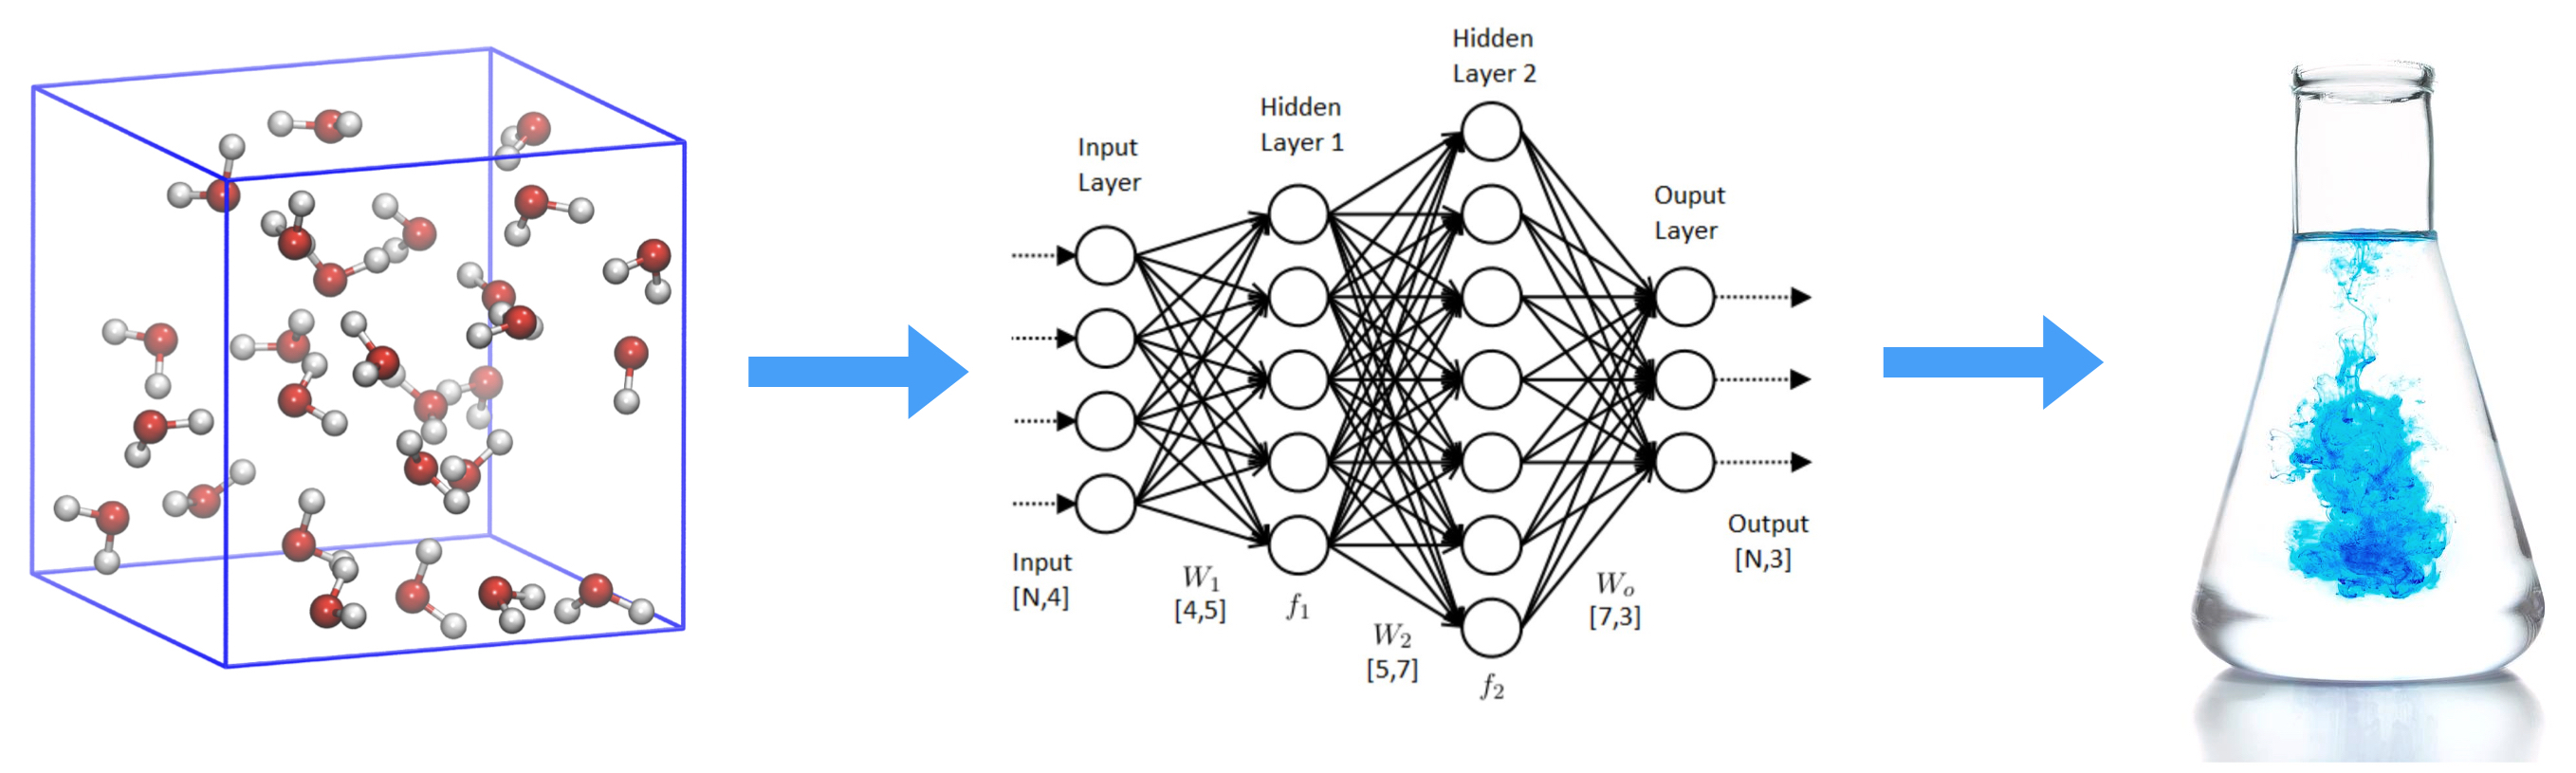
\includegraphics[scale=0.17]{latex_files/Picture.jpeg}
\end{center}
\vspace{1cm}
\begin{center}
    Veronika JURÁSKOVÁ \\
    Frédéric CELERSE \\
    Rubén LAPLAZA \\
    Clémence CORMINBOEUF
\end{center}
%\vspace{2cm}
%\begin{mybox1}{}
%\Warning Please visit the website: \url{https://toto-is-coming-soon} to obtain last updates of this tutorial and information about other new tutorials.
%\end{mybox1}
 
% FIN PAGE DE PRESENTATION

% TABLE DES MATIERES
\newpage
\tableofcontents

% DEBUT DU TUTORIEL
\newpage
% SECTION INTRODUCTION
\pagestyle{fancy}
\renewcommand\headrulewidth{1pt}
\fancyhead[R]{MD combining NN: tutorial}
\renewcommand\footrulewidth{1pt}
\fancyfoot[C]{\thepage}
\fancyfoot[R]{\today}
\section{Introduction}
\fancyhead[L]{1. Introduction}
This tutorial aims to guide the building of neural network-based potentials (NNPs) and their application in molecular dynamics (MD). As the \textit{ab initio} MD is too computationally demanding to obtain statistically converged simulations of chemical reactions and processes in large systems, the MD with NNPs benefits from the much lower cost of the simulation while the accuracy of the AIMD is conserved.  
In this regard, NNPs have been already used in the reactive simulations in the gas phase and aqueous solutions (\textit{e.g.}, in the description of proton transfer and urea hydrolysis). 

\textbf{Part 1} of this tutorial is dedicated to the generation of the Behler-Parrinello NNPs, including the preparation of a robust data set, selection of the descriptors, and monitoring of the accuracy of the training. \textbf{Part 2} demonstrates how to use the NNPs using the i-Pi interface to LAMMPS and other codes. \textbf{Part 3} introduces the concept of baselined NNPs and showcases its advantages compared to NNPs trained directly on DFT data. 
\fancyhead[L]{2. Neural Networks-based potentials: Crash course}

\section{Neural Networks-based potentials: Crash course}

\textbf{Neural Networks are statistical models which can reproduce complex non-linear functions using large amounts of the training points.} The availability of so-called \textit{Big data} in a broad range of human activities resulted in the harvesting of neural networks in the development of game-playing models, speech and text recognition software, or analysis of patients' data in modern health care, to name a few. Recently, the power of NN to reproduce highly complex data has been exploited in the development of a new generation of potentials for molecular dynamics. The Neural Network Potentials (NNPs) are trained to mimic the shape of the corresponding potential energy surface using the \textbf{data sets} containing coordinates and corresponding \textit{ab initio} data (i.e., energy and possibly forces). The resulting NNPs are then used to propagate molecular dynamics with the accuracy of the underlying \textit{ab initio} method but with a fraction of its original cost. Many NN architectures to train the NNPs have been proposed during the last years. In this tutorial, we focus on the training of Behler-Parrinello NNPs based on feedforward NN.  

\subsection{Feedforward Neural Networks}
\begin{figure}[!h]
    \centering
    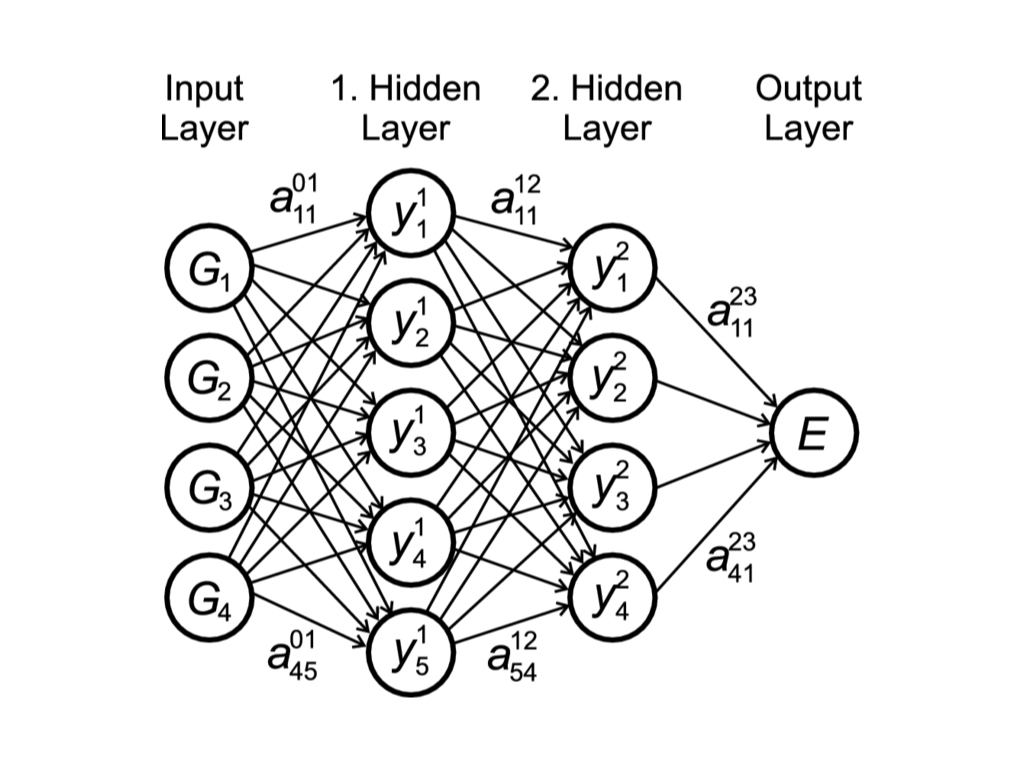
\includegraphics[scale=0.4]{latex_files/NNP_scheme.jpeg}
    \caption{Schematic representation of a small feedforward NN. Nodes are interconnected in order to establish a functional relation between a set of coordinates $G$ (input layer) and the potential energy of the structure E (output layer). }
    \label{NNP_scheme}
\end{figure}
The example of the feedforward NN is depicted in Fig. \ref{NNP_scheme}. It is made from several nodes organized in interconnected layers. The potential energy \textit{E} corresponds to the node in the \textbf{output layer} and the atomic coordinates of a frame are provided in the \textbf{input layer} as vectors of input coordinates $G=\{G_i\}$. The input and output layers are connected via several so-called \textbf{hidden layers} with no physical meaning. The number of layers and the nodes define the flexibility of the final NN. The example shows the NN with two layers containing five and four nodes, respectively. 
Each node is connected to the nodes of the next layer with a specific weight \textbf{$a_{ij}^{kl}$}, where $i$ is the index of a node of layer $k$, which is connected to the node with index $j$ of layer $l$. For instance, the $a_{45}^{01}$ connects the nodes $G_4$ ($k = 0$, $i=4$) and $y_5^1$ ($l=1$,  $j=5$). Nodes in hidden and output layers are connected to a so-called bias node, which scales their values by a bias weight b$_i^j$, where $j$ is the layer of the target node and $i$ is the node index. In our scheme, the bias node is omitted for simplicity.

The value y$_i^j$ of any node is computed as:
\begin{equation}
    y_i^{j} = f_i^j(b_i^j + \sum_{k=1}^{N_{j-1}} a_{k,i}^{j-1,j} y_k^{j-1})
\end{equation}
The equation is a linear combination of the values of all nodes in the previous layer scaled by the bias weight. The term f$_i^j$ represents the \textbf{activation function} of the NN. The activation function ensures the ability to fit complex non-linear functions. The examples of activation functions are:
\begin{itemize}
    \item hyperbolic tangent,
    \item sigmoid function,
    \item Gaussian function,
    \item Softplus
    \item trigonometric functions
    \item exponential function.
\end{itemize}
According to Figure~\ref{NNP_scheme}, the complete functional form for the energy is given by:
\begin{equation}
    E = f_1^3(b_1^3 + \sum_{k=1}^4 a_{k1}^{23} f_k^2 (b_k^2 + \sum_{j=1}^5 a{jk}^{12} f_j^1 (b_j^1 + \sum_{i=1}^4 a_{ij}^{01} G_i)))
\end{equation}

\subsection{High--dimensional NNP}
\begin{figure}[!htp]
    \centering
    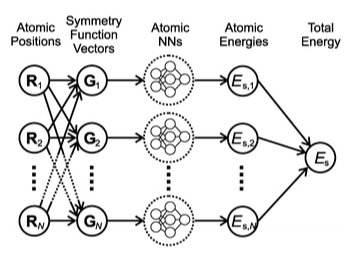
\includegraphics[scale=0.7]{latex_files/High-dimensional-NNP_scheme.jpeg}
    \caption{High dimensional NN scheme: Atomic positions are represented by a vector of symmetry functions $G_i$. }
    \label{High-dimensional-NNP_scheme}
\end{figure}
Feedforward neural networks discussed in the previous section suffer from several drawbacks preventing their application in the simulation of complex chemical systems. The limitations are, for instance:
\begin{enumerate}
    \item absence of symmetry between equivalent terms (for instance, the OH bonds of a water molecule)
    \item system size dependency: no atoms could be deleted or added as it causes problems in the connecting weights.
\end{enumerate}
In 2007, Behler and Parrinello proposed a solution to this problem by expressing the total energy $E_s$ as a sum of the atomic energy contributions E$_i$.\cite{Behler2007}
\begin{equation}
    E_s = \sum_{i=1}^{N_{atom}} E_i
\end{equation}
Starting from the Cartesian coordinates $R$, every atom is represented by a set of atom-centered symmetry functions $G_i$, which describe the atoms' chemical environment within a given cutoff. Each atom is then assigned a feedforward NN yielding the atomic contribution to the total energy. The weights of the NN are identical for atoms of the same element to ensure that the trained NNPs do not depend on the number and order of the atoms.

\subsection{Atom-centered symmetry functions}

Together with the NN topology, the seminal work of Behler and Parrinello introduced also new types of symmetry functions to characterize the local environment of each atom. The so-called Atom-centered symmetry functions (ACSFs)\cite{behl11jcp} are constructed from the positions of the atoms and their closest neighbors. This representation guarantees that the atoms with the same environment yield the same atomic energy contribution which is also translationally and rotationally invariant. 

The typically used ACSFs are two-body radial and three-body angular functions in a form:

\begin{equation}
    G_i^2  = \sum_i e^{-\eta (R_{ij}-R_s)^2} \cdot f_c(R_{ij}) \label{eq:radial}
\end{equation}
\begin{equation}
    G_i^3  = 2^{(1-\xi)} \sum_{j,k \neq i}^{\mathrm{all}}(1 + \lambda \mathrm{cos}\;\theta_{ijk})^{\zeta} \cdot e^{-\eta (R_{ij}^2 + R_{ik}^2 + R_{jk}^2)} \cdot f_c(R_{ij}) \cdot f_c(R_{ik}) \cdot f_c(R_{jk}),
    \label{eq:angular}
\end{equation}

where $f_c$ is a cutoff function ensuring the smooth decay of the symmetry function to zero.   

In this tutorial, we use the original Behler-Parrinello ACSFs. However, during the last years, many modifications to the original ACSFs were proposed as well as new types of functional forms to describe the atomic environments. Various types of structural representations are summarized for example in Ref. \citenum{Musil2021}.

\subsection{Constructing and training NN}
The general protocol to construct NNP is as follows:
\begin{enumerate}
    \item \textbf{Define an initial set of structures and compute the reference energies and forces.} The electronic structure method used as a reference should be accurate enough to describe the studied problem.
    \item T\textbf{rain the first version of NNPs.} The fraction of the data set (\textit{e.g.} 80 \%) is used in the NNP training (so-called training set) while the remaining part serves as a test set to validate the error on unseen data. Ideally, several different NNP with different training sets should be trained to identify potential problems in the training set.
    \item \textbf{Perform preliminary simulations using the NNPs} to evaluate the stability of the NNP and identify underrepresented areas of the PES, \textit{e.g.} structures triggering extrapolation warnings or unphysical geometries.
    \item \textbf{Isolate the problematic structures}, compute reference data and add them to the training set and re-train the NNP.
    \item Repeat the validation and re-training of the NNP until no instabilities are present.
\end{enumerate}

For a detailed general tutorial review on Behler-Parrinello NN, see Ref. \citenum{Behler2015tutorial}. 

\newpage
\fancyhead[L]{3. Requirements}
\section{Requirements}
This tutorial presents a workflow that requires an extensive number of different software packages, scripts, and libraries. The versions of the codes used here are listed below.
\subsection{Software}
All the codes are available at GitHub (see the last section of tutorial):
\begin{itemize}
    \item n2p2 (version 1.0.0)
    \item LAMMPS (version 2)
    \item i--PI (version 2.0)
    \item Tinker (version 8.8)
    \item cp2k (version 6.1)
\end{itemize}

\subsection{Dependencies}
\begin{itemize}
    \item python (version 2.7 and 3.6)
    \item libraries intel, intel-mpi, intel-mkl, gsl, eigen, gc,c mvapich2, openblas, n2p2/lib
\end{itemize}

\newpage

\fancyhead[L]{4. Building NNPs}
\section{Part 1: How to generate neural network potentials}
\subsection*{Instructions}

Currently, there is no universal NNP that is applicable to model all classes of systems. Despite the ongoing efforts in the training of general neural network-based force fields, many systems require building the NNPs from scratch. In the following section, we provide general instructions on how to train NNP using the Behler-Parrinello approach. The required steps include: 

\begin{enumerate}
    \item Sampling of the phase space to produce initial training structure;
    \item Generating a large pool of symmetry functions;
    \item Identification of a representative set of fingerprints;
    \item Careful selection of a small set of structures for the training of NN;
    \item Computation of reference forces and energies for the selected structures;
    \item Training of the NN.
\end{enumerate}

The training protocol is summarized in the Fig. \ref{protocol}.
\begin{figure} [!htp]
    \centering
    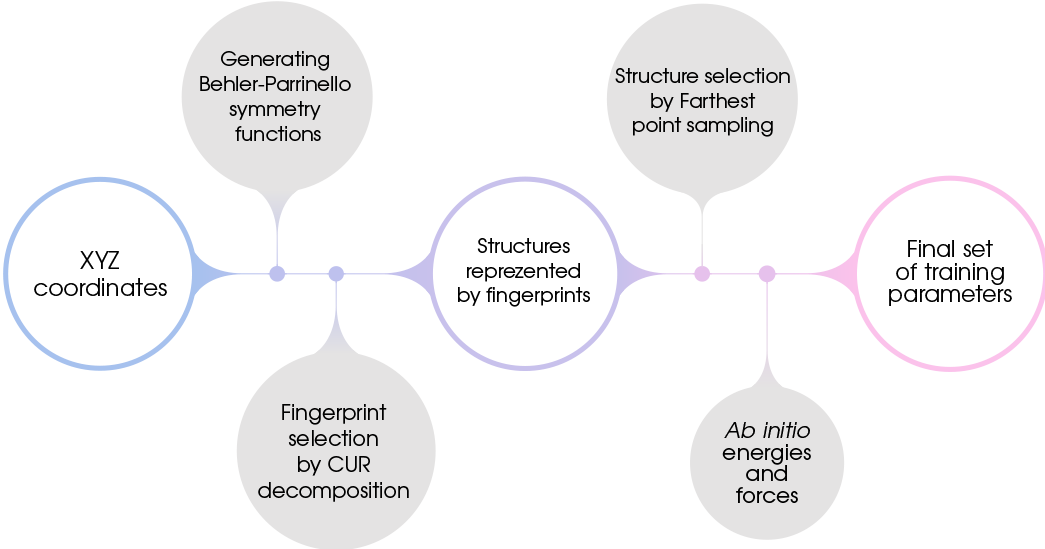
\includegraphics[scale=1.5]{latex_files/protocol.png}
    \caption{Scheme of the NNP preparation.}
    \label{protocol}
\end{figure}

\newpage
\subsection{Step 0: The system}
\begin{figure} [!htp]
    \centering
    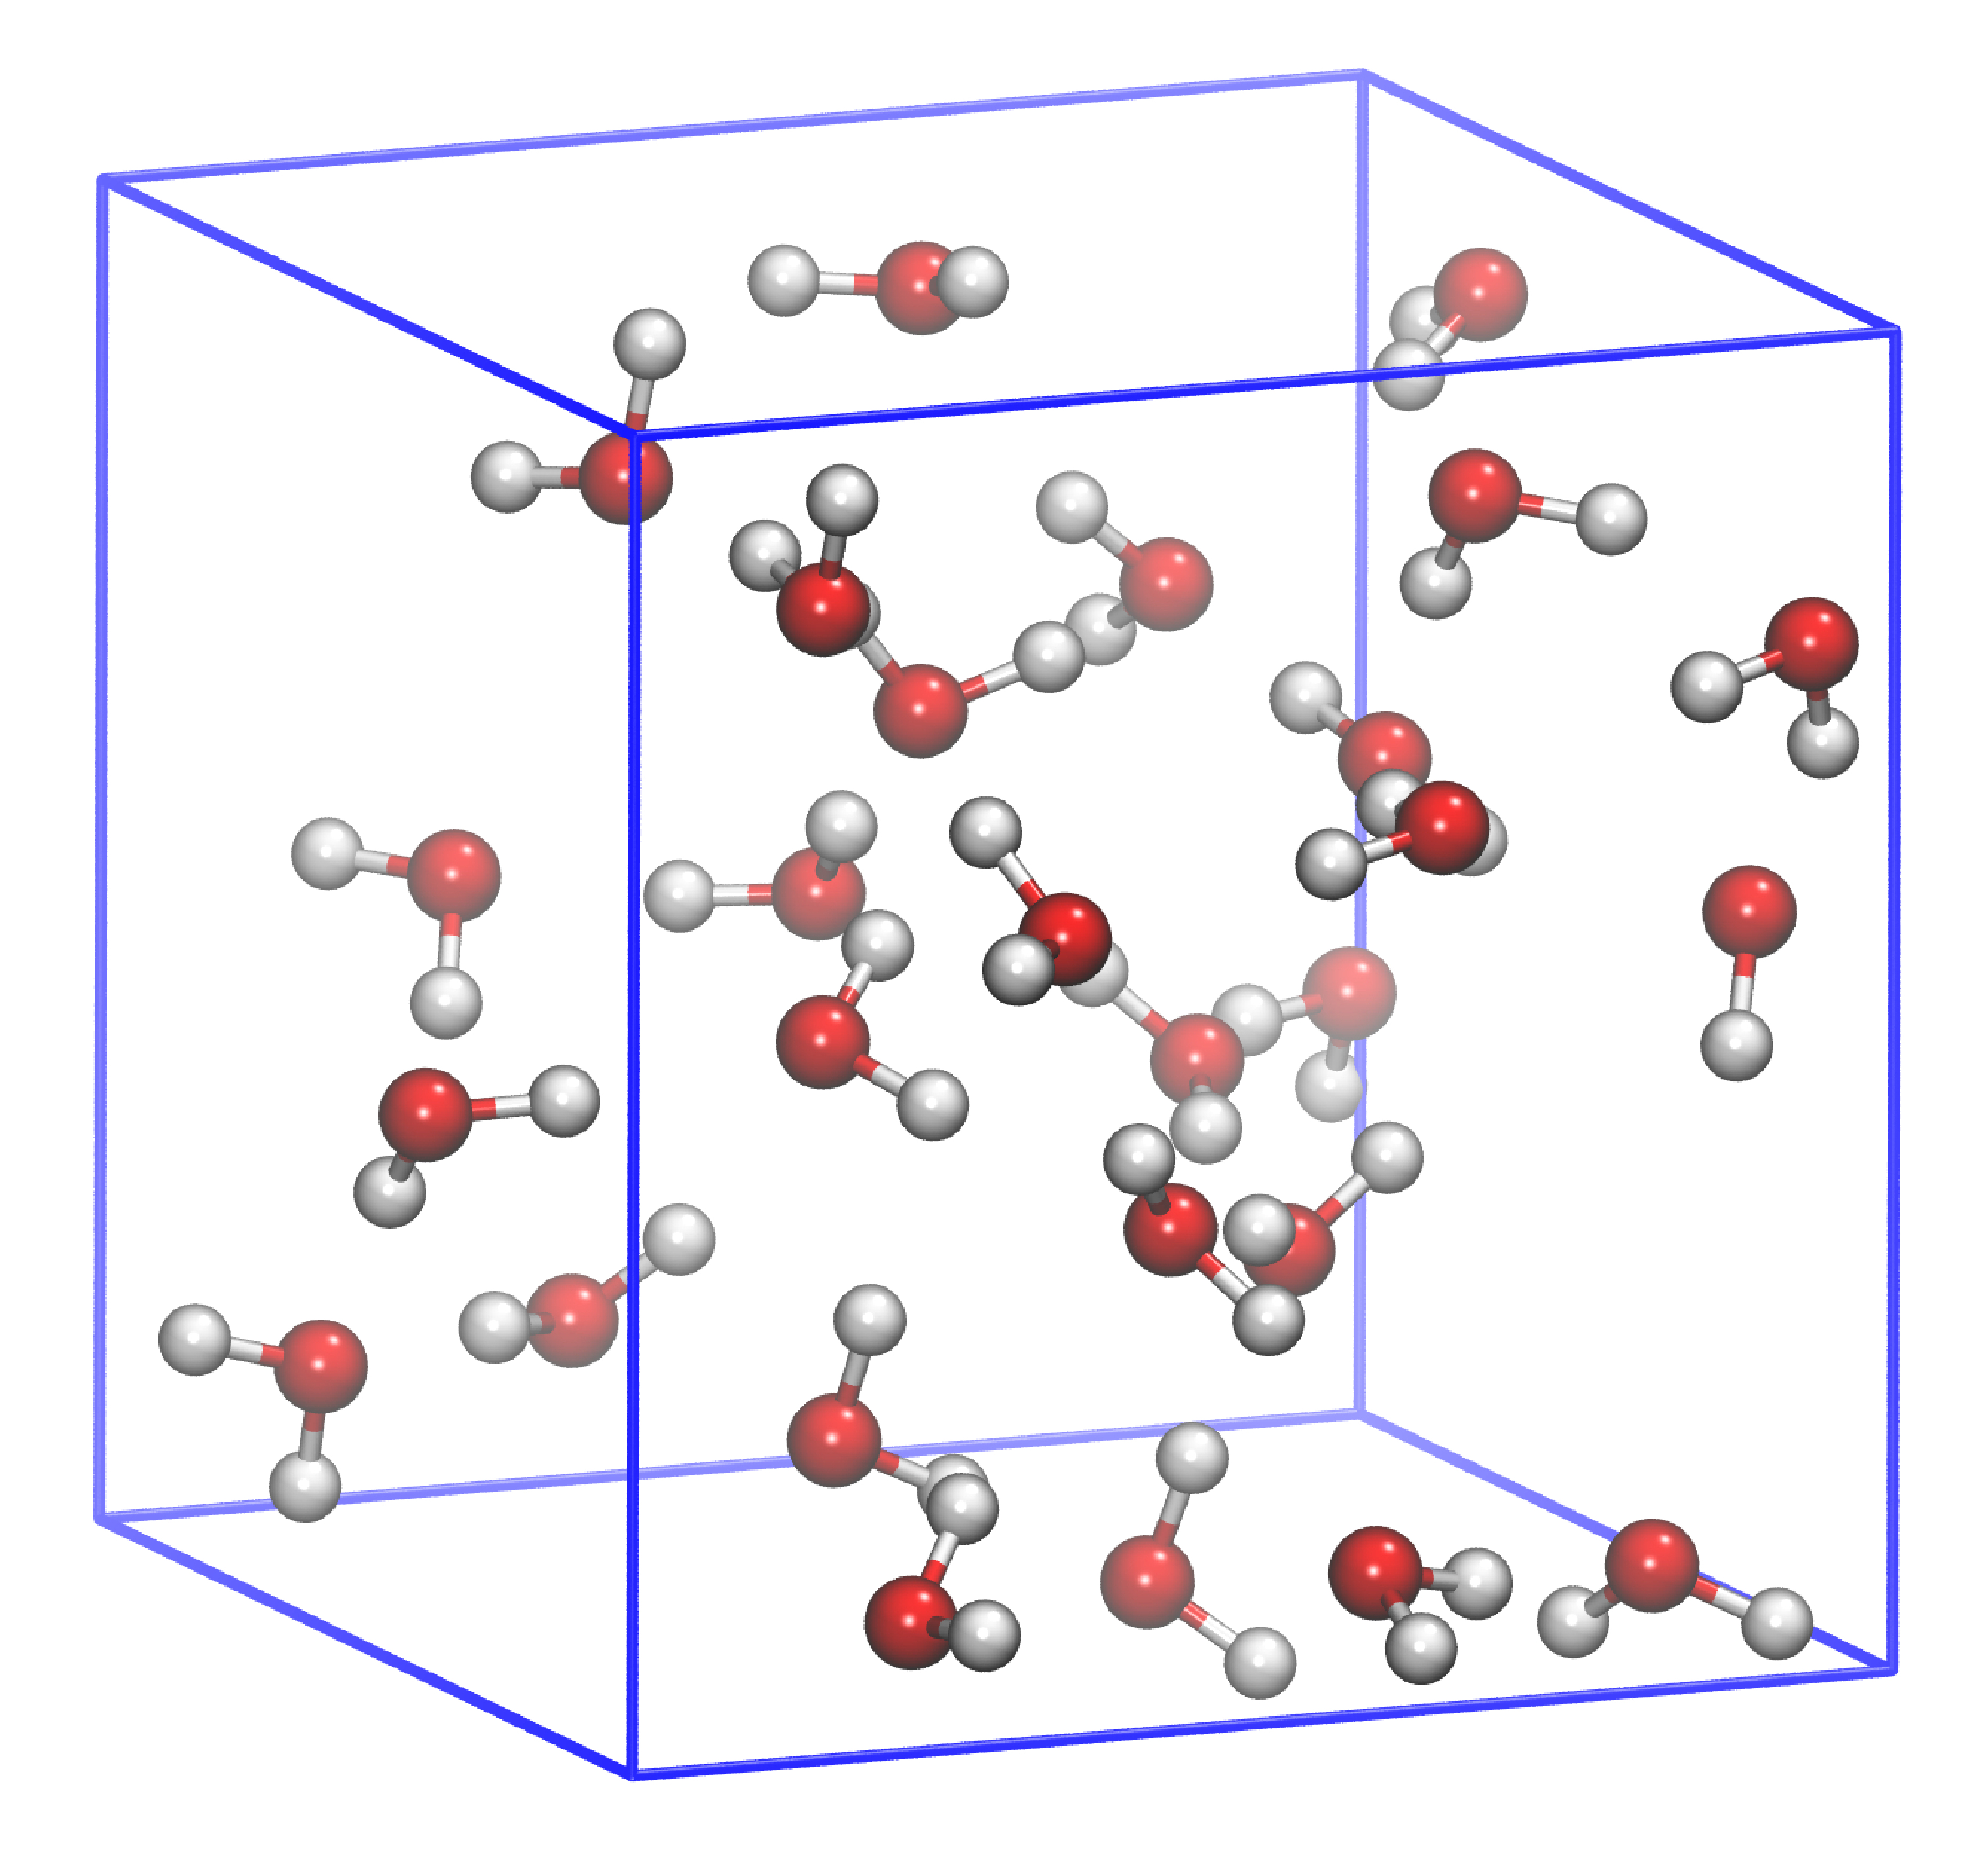
\includegraphics[scale=0.05]{latex_files/watertiny.jpeg}
    \caption{System containing 27 molecules in a cubic box with edge of 9.32 \AA.}
    \label{Rep_sys}
\end{figure}

As a relatively simple test case, we train the NNPs for a small water box containing 27 water molecules with a cell size of 9.32 \AA. These systems are composed of only two elements, \textit{i.e.} H and O, which significantly simplifies the training.

\subsection{Step 1: Generating the data}
\begin{mybox2}{{Files needed}}
\begin{minipage}[c]{0.5\linewidth}

\includegraphics[scale=0.2]{latex_files/tinker.png}
\end{minipage}
\begin{minipage}[c]{0.5\linewidth}
\begin{itemize}
    \item system.xyz
    \item system.key
    \item system.dyn
    \item water03.prm
    \item \textit{dynamic} module
\end{itemize}
\end{minipage}
\end{mybox2}

The first step in the tutorial is the preparation of the training set. The training set can contain systems of different sizes and different compositions. To keep things simple, we will train the NNPs using only one size of the water box. To generate an extensive set of the structures, it is beneficial to use molecular dynamics starting either from equilibrated structure or from experimental data (\textit{e.g.}, X-ray). Random displacement of the atoms could be also applied.

As the first training set should be large enough and contain representative geometries, the potential for the exploratory dynamics should provide a reasonable cost/accuracy ratio. For example, classical force fields might not be the best choice, as they can sample structures that are too different from the ones obtained at the reference level. The suitable compromise is, therefore, the application of semiempirical methods or polarizable force fields.

Herein we generate the system using AMOEBA polarizable force-field as available in Tinker. The files required for the simulation are *.xyz,  *.key, and *.prm. For more information on the preparation of the files for Tinker, see tutorials listed in section \ref{sec:tutorials}.

The files contain:

\begin{itemize}
    \item The *.xyz file - the Cartesian coordinates of the initial water box in the Tinker xyz format (Caution! Tinker xyz differs significantly from standard xyz or extended xyz formats.)  
    \item The *.key file - the settings to run the dynamics.
    \item The *.dyn - positions, velocities, and accelerations of the last frame of the dynamics.
    \item The *.prm file - AMOEBA parameters (all the terms to compute the potential energy of a specific structure)
\end{itemize}

MD using Tinker can be launched as:
\begin{center}
\mybox{\textit{dynamic system 1000000 2.0 1 2 300 $>$ system.out}}
\end{center}

This command means that the simulation will run using the \textit{dynamic} module of Tinker for 1000000 steps with a time step of 2.0 fs (\textit{i.e.}, the total length of the simulation is 2 ns). The next term specifies the frequency (in ps) of saving the trajectory to the *.arc file (here we save it every 1 ps). The final \textit{system.arc} file will thus contain 2000 frames. The following term specifies the mode of the dynamics, 2 corresponds to NVT canonical ensemble. The last term corresponds to the simulation temperature (300 K). 

\begin{mybox1}{Enhanced sampling}
\Warning As the system is quite simple, the standard molecular dynamics are sufficient to provide an extensive sampling. In more complex cases, however, the simulations starting from different initial structures or using enhanced sampling techniques might be needed to ensure that all the relevant structures are present in the training set. Suitable simulations techniques include, for instance:
\begin{enumerate}
    \item Replica exchange molecular dynamics
    \item Sampling techniques using bias, such as metadynamics, steered molecular dynamics, umbrella sampling, ...
    \item Transition path sampling
\end{enumerate}
\end{mybox1}
\begin{mybox1}{Extending the database with more distorted structures}

\Warning The NNPs have in general very limiting extrapolation capacity. As they are trained only on the information included in the training set, it is beneficial to consider more distorted structures covering the repulsive and dissociative parts of the PES. Distorted structures can be generated by simulations using, for example: 
\begin{enumerate}
    \item High temperature
    \item High pressure
    \item Path integral molecular dynamics
    \item Specific constraints and restraints
    \item Random displacement
\end{enumerate}

\end{mybox1}
\begin{mybox3}{Output Files}
\begin{itemize}
    \item system.out
    \item \textbf{system.arc} (file containing the structures)
    \item system.dyn
\end{itemize}
\end{mybox3}

\subsection{Step 2: Descriptor selection}
To assign the structures with a suitable set of descriptors, we generate a large pool of the ACSFs and select a small representative set using, for example, CUR decomposition.

\subsubsection{Generating symmetry functions}
\begin{mybox2}{{Input Files, Executables and Scripts}}
\begin{minipage}[c]{0.5\linewidth}

\includegraphics[scale=0.1]{latex_files/Python-fortran.jpeg}
\end{minipage}
\begin{minipage}[c]{0.5\linewidth}
\begin{itemize}
    \item system.arc
    \item \textcolor{red}{from\_txyz\_to\_n2p2.f90}
    \item \textcolor{red}{symmetry\_functions.py}
\end{itemize}
\end{minipage}
\end{mybox2}

As a first step, place the structures generated in the previous part to the \textit{system.arc} file. 

Structures in this file can be converted to input files for n2p2 as follows:

\begin{enumerate}
    \item compile the fortran code \textcolor{red}{from\_txyz\_to\_n2p2.f90}:
    \textit{gfortran from\_txyz\_to\_gen.f90 -o from\_txyz\_to\_gen} 
    \item place the system.arc file in the same directory of the \textcolor{green}{from\_txyz\_to\_gen} executable and launch it as \textit{./from\_txyz\_to\_gen}
\end{enumerate}
The script generates input.data file for the n2p2. The definition of each frame starts with a short header:
\vspace{0.5cm}
\begin{verbatim}
begin
comment 
lattice 17.612 0.0 0.0 
lattice 0.0 17.612 0.0 
lattice 0.0 0.0 17.612 
\end{verbatim}
\noindent "lattice" defines the dimension of the box in Bohr.
Each atom of the structure is defined as: \\
\begin{verbatim}
 atom     -4.367    5.267     4.603   O   0 0   0.0  0.0  0.0  
 \end{verbatim}
The keyword "atom" specifies that the line corresponds to one atom, -4.367, 5.267, 4.603 are the xyz coordinates of the atom in Bohr, O is the element label, the following two columns 0 0 are not used. Finally, the last three columns 0.0 0.0 0.0 are the xyz force components acting on the atom. In this example, forces are set to 0.0 since they are not used.
\vspace{0.5cm}

 \noindent The frame ends with: 
\vspace{0.5cm}

\begin{verbatim}
energy 0.000 
charge 0.0 
end 
\end{verbatim}

\noindent where "energy" is the reference total energy of the system, "charge" is the total charge of the system, and "end" closes the definition of the structure. 

\begin{mybox1}{Units in n2p2}
\Warning As indicated on the n2p2 website, the units correspond to the physical units defined in the input files. As we combine several codes with possibly different unit specifications, keep track of the units and stay consistent within the workflow.

In the inputs for n2p2, we use:
\begin{enumerate}
    \item lattice: \textbf{Bohr}
    \item x/y/z positions: \textbf{Bohr}
    \item x/y/z forces: \textbf{Hartree Bohr$^{-1}$}
    \item energy: \textbf{Hartree}
\end{enumerate}

\textcolor{red}{The conversion from Angström to Bohr is done by a multiplication by a factor \textbf{1.88973}}
\end{mybox1}

All settings and parameters for the training of NNP are specified in \textbf{input.nn} file. It contains three main parts:
\begin{enumerate}
    \item GENERAL NNP SETTINGS
    \item ADDITIONAL SETTINGS FOR TRAINING
    \item SYMMETRY FUNCTIONS
\end{enumerate}

GENERAL NNP SETTINGS specify the general set-up of the neural network, for instance, a number of the elements, layers and nodes, cut-offs, scaling normalization, etc.

ADDITIONAL SETTINGS FOR TRAINING define explicitly the parameters of the training as the number of epochs, fraction of energies used in the training, and type of the optimizing algorithm. 

The last part defines the symmetry functions sets used in training. While the parameters for the training can be found in the literature and possible modification directly depend on the simulated system, the symmetry functions are often built completely from scratch and require careful selection.

The n2p2 currently supports Behler-Parrinello types of symmetry functions (radial, angular, wide angular, for definition see Ref. \citenum{behl11jcp}), their weighted variants (Ref. \citenum{Gastegger2018}) and polynomial symmetry functions (Ref. \citenum{Bircher2021}). In this tutorial, we use standard Behler-Parrinello functions.

The initial set of the symmetry function can be generated, for example, by a \textit{symfunc\_paramgen.py} code by Florian Buchner available at \url{https://github.com/flobuch/n2p2/tree/symfunc_paramgen}. Jupyter notebook with an example of the use of the code is provided at \url{https://github.com/flobuch/n2p2/blob/symfunc_paramgen/tools/python/symfunc_paramgen/examples/example.ipynb}.

For the NNP of the water box, we generate a set of radial symmetry functions with cutoff $r_c = 4, 8, 12$ Bohr and $N = 8$ and two sets of angular symmetry functions following the protocol described in Ref. \citenum{Imbalzano2018}.  Store the symmetry functions in one file \textit{e.g.},  asfs.txt and append it at the end of the input.nn.

\begin{center}
\mybox{\textit{cat asfs.txt $>>$ input.nn}}
\end{center}


The initial input files needed for the training are therefore:
\begin{itemize}
    \item \textbf{input.data}
    \item \textbf{input.nn}.
\end{itemize}

\begin{mybox3}{Output Files}
\begin{itemize}
    \item \textbf{input.data}
    \item \textbf{input.nn} 
\end{itemize}
\end{mybox3}

\subsubsection{Selection of a subset of descriptors}
\begin{mybox2}{{Input Files, Executables and Scripts}}
\begin{minipage}[c]{0.5\linewidth}

\includegraphics[scale=0.1]{latex_files/n2p2.png}
\end{minipage}
\begin{minipage}[c]{0.5\linewidth}
\begin{itemize}
    \item input.data
    \item input.nn
    \item \textcolor{green}{nnp--scaling}
\end{itemize}
\end{minipage}
\end{mybox2}
Using the symfunc\_paramgen tool, we generated 192 radial and 768 angular symmetry functions, \textit{i.e.}, 480 SF per element. The goal of this section is to select a small subset of the SF that will be used for the training of the NNPs. Following the benchmark and recommendations discussed in Ref. \citenum{Imbalzano2018}, we use the CUR decomposition scheme to select 64 unique symmetry functions per element. The details of CUR and more advanced CovCUR techniques can be found in Ref. \citenum{maho-drin09pnas,Imbalzano2018,Cersonsky2021}. 

To evaluate the symmetry functions over the geometries, we use \textit{nnp-scaling} tool in n2p2. However, the number of the symmetry function is huge and the storage of the values over the whole set of structures would be memory demanding. We therefore randomly select a subset of structures from the original input.data file using \textit{nnp-select} tool.

\begin{center}
\mybox{\textit{nnp-select random 0.05 123}}
\end{center}

Keyword \textit{random} indicates the random selection of the structures, 0.05 corresponds to the percentage of selection, and 123 is the seed for the random generator. Modify the percentage so it corresponds to roughly 1000 structures.

Finally, evaluate the symmetry functions by \textit{nnp-scaling}. Regarding the computational cost, it is advisable to submit the scaling on cluster in parallel, for example:

\begin{center}
\mybox{\textit{mpirun -n 8 nnp-scaling 500 $>$ logfile}}
\end{center}


\textit{nnp-scaling} generates three output files:
\begin{enumerate}
    \item \textbf{logfile}: contains a list of the symmetry functions and their parameters. \textbf{Needed for the CUR selection.}
    \item \textbf{function.data}: the evaluation of all the symmetry functions over the data in \textit{input.data}. \textbf{Needed for CUR selection.}
    \item \textbf{scaling.data}: statistic of the symmetry functions, \textit{i.e.}, the minimum and maximum values, mean and sigma.
\end{enumerate}

TO BY ADDED!!

\subsection{Step 3: Hybrid DFT force--energy computations}
\begin{mybox2}{{Input Files, Executables and Scripts}}
\begin{minipage}[c]{0.5\linewidth}

\includegraphics[scale=0.1]{latex_files/Python-fortran.jpeg}
\end{minipage}
\begin{minipage}[c]{0.5\linewidth}
\begin{itemize}
    \item landmarks.dat
    \item input.data
    \item \textcolor{red}{selection.f90}
    \item \textcolor{red}{from\_data\_to\_xyz.f90}
    \item \textcolor{red}{from\_xyz\_to\_cp2k.f90}
\end{itemize}
\end{minipage}
\end{mybox2}

From the landmarks.dat file generated in the previous step, we need to extract structures for the single point reference computations, for example using \textcolor{red}{selection.f90}:

\begin{center}
\mybox{\textit{gfortran selection.f90 -o selection ; ./selection}}
\end{center}
It will generate a new file \textbf{new--input.data} containing the 1000 structures selected by the FPS. In this tutorial, we use cp2k code to generate energy and forces of the water box. However, the reference computations for the NNP in general do not need to be periodic. The geometry input files for cp2k can be generated by: 

\begin{enumerate}
    \item \textit{gfortran from\_data\_to\_xyz.f90 -o from\_data\_to\_xyz ; ./from\_data\_to\_xyz}
    \item \textit{gfortran from\_xyz\_to\_cp2k.f90 -o from\_xyz\_to\_cp2k ; ./from\_xyz\_to\_cp2k}
\end{enumerate}

\begin{mybox3}{Output Files}
\begin{itemize}
    \item \textbf{\$i-cp2k.xyz}
\end{itemize}
\end{mybox3}

\subsubsection{CP2K computations}
\begin{mybox2}{{Input Files, Executables and Scripts}}
\begin{minipage}[c]{0.5\linewidth}

\includegraphics[scale=0.1]{latex_files/CP2K_logo.png}
\end{minipage}
\begin{minipage}[c]{0.5\linewidth}
\begin{itemize}
    \item \$i-cp2k.xyz
    \item input.cp2k
    \item \textcolor{red}{prep-file.sh}
\end{itemize}
\end{minipage}
\end{mybox2}

The cp2k computations can be automatized by \textcolor{red}{prepare.sh} script which automatically creates directories for the computations (one per structure). The directories contain geometry files and inputs to cp2k. Here, we use the CP2K 6.1 version to perform reference energies and forces computations at the PBE--D3BJ level of theory. All elements are described with the TZV2P--MOLOPT basis set with cores represented by the dual--space Goedecker--Teter--Hutter pseudopotentials (GTH PBE). The plane--wave cutoff is set to 700 Ry with a relative cutoff of 70 Ry.\\

Launch a cp2k computations following the installation of your machine. For example:
\begin{center}
\mybox{\textit{cp2k.popt -i input.cp2k -o output.cp2k}}
\end{center}
The output of the computation including energy and forces is in the output.cp2k file.
\\
\begin{mybox3}{Output Files}
\begin{itemize}
    \item \textbf{output.cp2k} 
\end{itemize}
\end{mybox3}
%
\subsubsection{Extraction of energy and forces}
\begin{mybox2}{{Input Files, Executables and Scripts}}
\begin{minipage}[c]{0.5\linewidth}

\includegraphics[scale=0.1]{latex_files/Python-fortran.jpeg}
\end{minipage}
\begin{minipage}[c]{0.5\linewidth}
\begin{itemize}
    \item output.cp2k
  \item \textcolor{red}{process.sh}
\end{itemize}
\end{minipage}
\end{mybox2}
The database of the energy and forces can be created using the process.sh scrip. The resulting information is saved in the database\_forces-pbe0.xyz file.
\\
\begin{mybox3}{Output Files}
\begin{itemize}
    \item \textbf{database\_forces-pbe0.xyz}
\end{itemize}
\end{mybox3}
%
\subsubsection{Final input.data file}
\begin{mybox2}{{Input Files, Executables and Scripts}}
\begin{minipage}[c]{0.5\linewidth}

\includegraphics[scale=0.1]{latex_files/Python-fortran.jpeg}
\end{minipage}
\begin{minipage}[c]{0.5\linewidth}
\begin{itemize}
    \item input.data
    \item database\_forces-pbe0.xyz
    %\item \textcolor{red}{update.f90}
\end{itemize}
\end{minipage}
\end{mybox2}
Finally, with the database of energies and forces for the training structures, we create the final input.data file which is used for the training. This can be done, for instance, by the XXX code.
\begin{center}
\mybox{\textit{gfortran update.f90 ; ./a.out}}
\end{center}
%You now have to replace your old input.data by the %\textbf{new-%input.data} generated as the output of your script for the %next step.
%\\
\begin{mybox3}{Output Files}
\begin{itemize}
    \item \textbf{input.data} 
\end{itemize}
\end{mybox3}
%
\subsection{Step 4: Neural Network Potentials}
%\subsubsection{New scaling.data file}
\begin{mybox2}{{Input Files, Executables and Scripts}}
\begin{minipage}[c]{0.5\linewidth}

\includegraphics[scale=0.1]{latex_files/n2p2.png}
\end{minipage}
\begin{minipage}[c]{0.5\linewidth}
\begin{itemize}
  \item input.data
   \item input.nn
     \item \textcolor{green}{nnp--scaling}
   \item \textcolor{green}{nnp--train}
\end{itemize}
\end{minipage}
\end{mybox2}
The last file we need to prepare for the training of the neural network is the preparation of the new scaling.data file. As in the previous case, we generate it using nnp-scaling in n2p2.

Finally, the training procedures can be launched. Depending on the system, the process can be parallelized and submitted, for example, as:
\begin{center}
\mybox{\textit{mpirun -n 32 nnp--train $>$ output.txt}}
\end{center}

The neural network potentials are trained to achieve as low RMSE on the test set as possible. The data to monitor the training behavior of the NNP are provided in the \textit{learning-curve.out} file. The file contains:
\begin{enumerate}
    \item Column 1: The index of the current epoch
    \item Column 2: RMSE of training energies per atom (physical units)
    \item Column 3: RMSE of test energies per atom (physical units)
    \item Column 4: RMSE of training forces (physical units)
    \item Column 5: RMSE of test forces (physical units)
\end{enumerate}

 The physical units correspond to the units used in the training data. In our case, energy is specified in Hartree (a.u.) and forces in Hartree per Bohr. The training errors discussed in the literature are commonly specified in the meV and meV/$\AA$ or kcal/mol and kcal/mol/$\AA$. The conversion factors are: 1 a.u = 627.5 kcal/mol = 27.211 eV, 1 Bohr = 0.529177 $\AA$. The learning curves can be plotted in Gnuplot to visualize the training progress. For example, the plotting of the RMSE in error in energy for the training set and test set:

\begin{center}
\mybox{\textit{p 'learning-curve.out' u 1:(\$2*1000*27.11) w l, 'learning-curve.out' u 1:(\$3*1000*27.11) w l }}
\end{center}

\begin{figure}
    \centering
    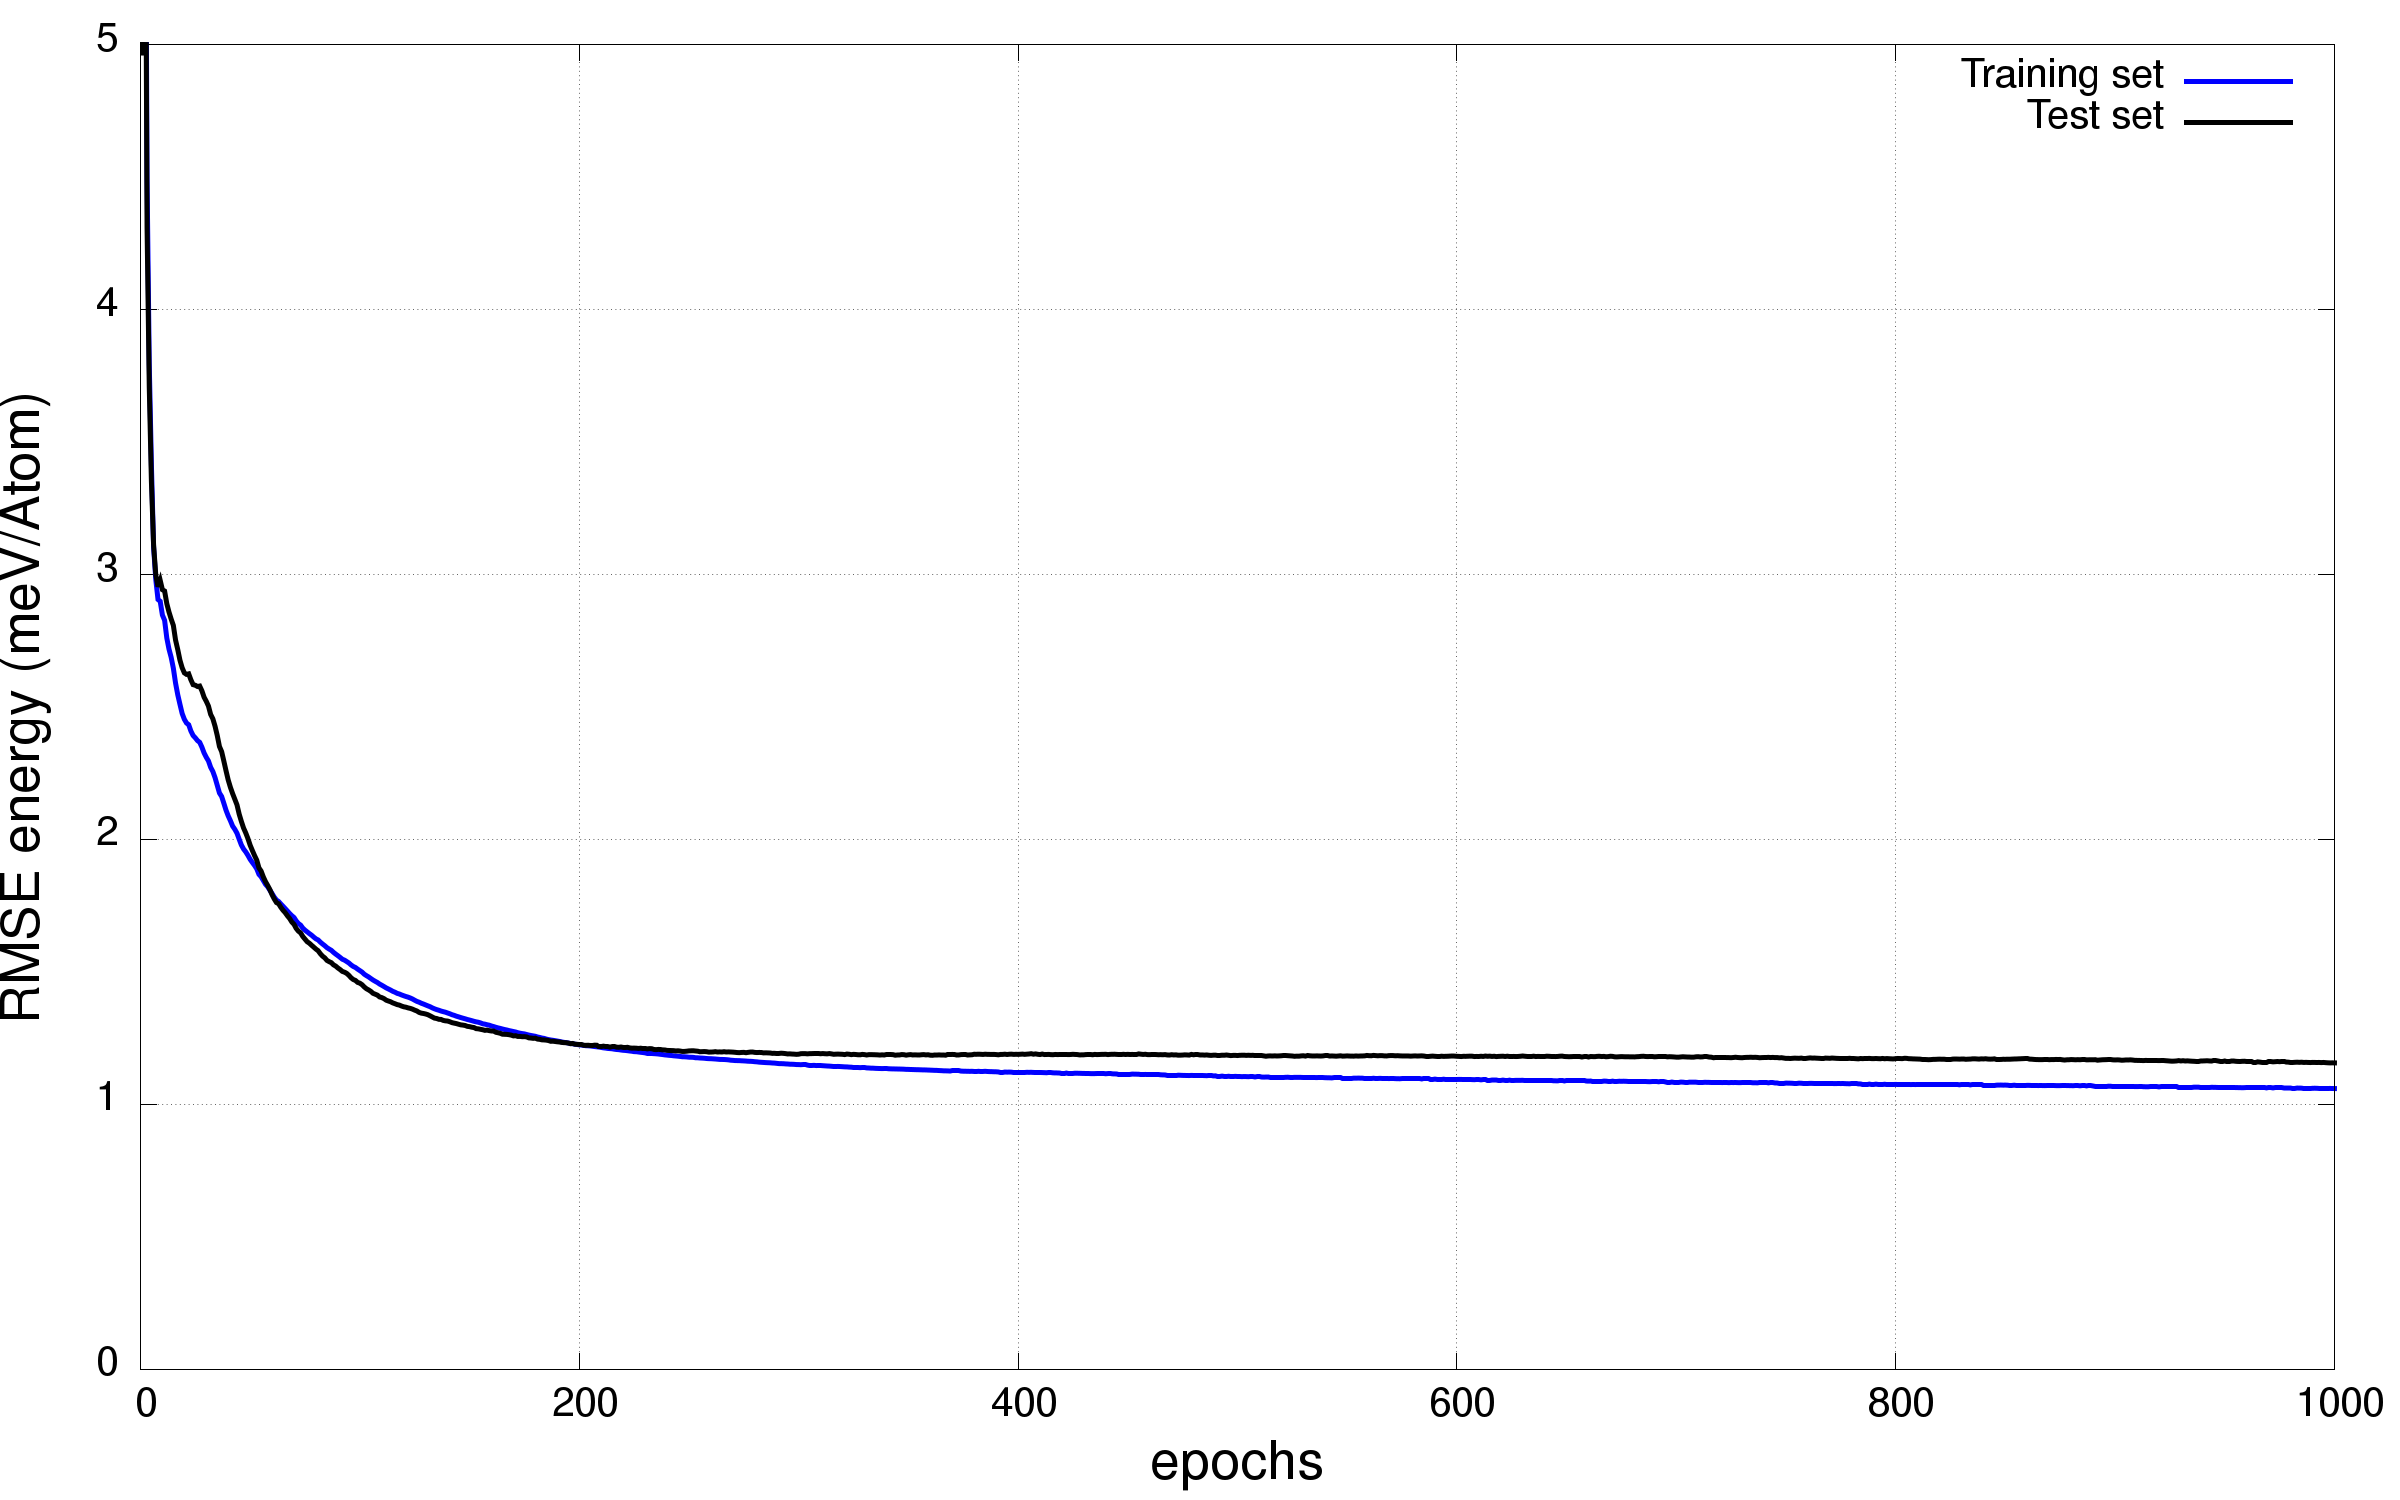
\includegraphics[scale=0.2]{latex_files/energy.png}
    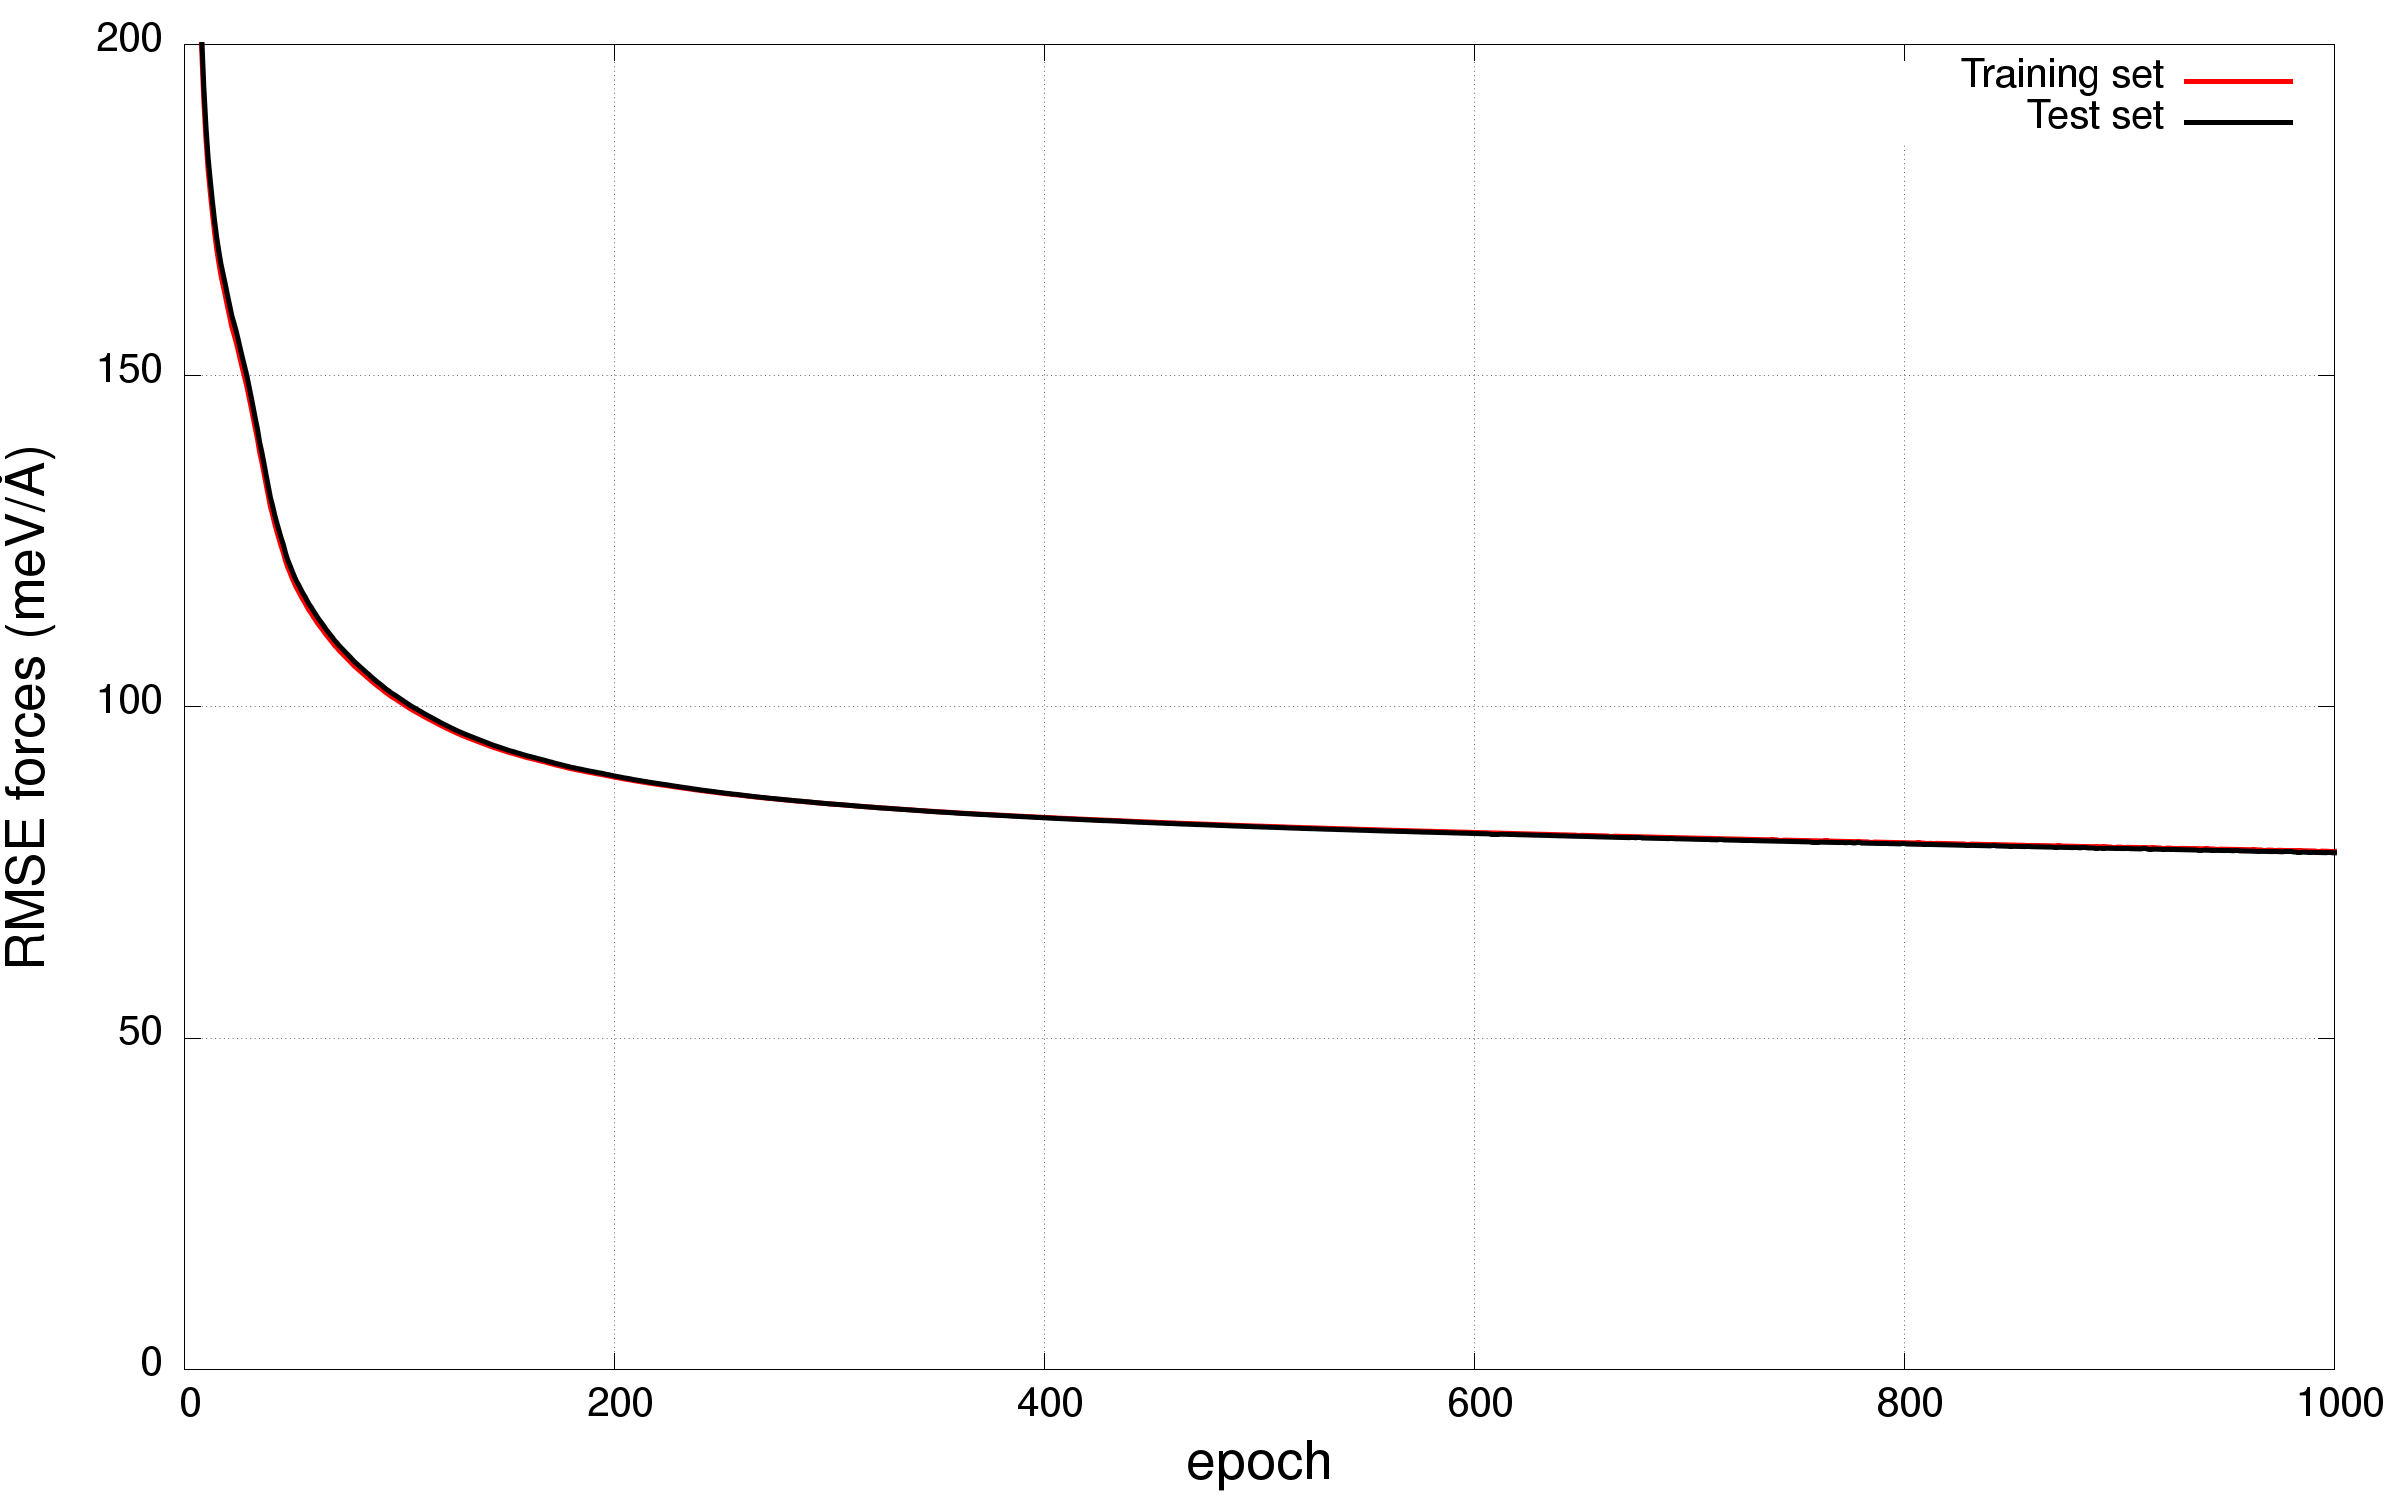
\includegraphics[scale=0.2]{latex_files/forces.png}
    \caption{Energy and forces learning curves. The training has been performed on 800 structures and testing on 200 structures.}
    \label{fig:my_label}
\end{figure}

The Behler-Parrinello NNP can often achieve RMSE around 1 meV/atom in energy and less than 100 meV/$\AA$ in forces. The RMSE obtained for the water box show a similar trend and can be tested in molecular dynamics.

\newpage
\fancyhead[L]{5. NNP--MD}
\section{Part 2: Application of NNP in Molecular Dynamics}
The stability of the NNP trained in the previous section should be verified in the molecular dynamics. To achieve this, we use a simulation workflow depicted in Fig. \ref{fig:workflow}. 

The workflow combines several existing approaches and codes representing a state-of-the-art method in molecular dynamics. The central part is the i-PI molecular dynamics driver, which propagates the nuclei using external potentials and guides the communication between all codes. 

The evaluation of the energy and forces for a given geometry is performed by the n2p2 library implemented in LAMMPS using the NNP we trained in the previous sections. The workflow allows to run MD with two types of NNPs: (i) direct NNPs (DNNP) reproducing the DFT data, and (ii) baselined NNPs (BNNP) (\textit{vide infra}) which serve as a correction applied on the top of a cheaper potential (\textit{e.g.}, a semiempirical method). 

\begin{figure}[!htp]
    \centering
    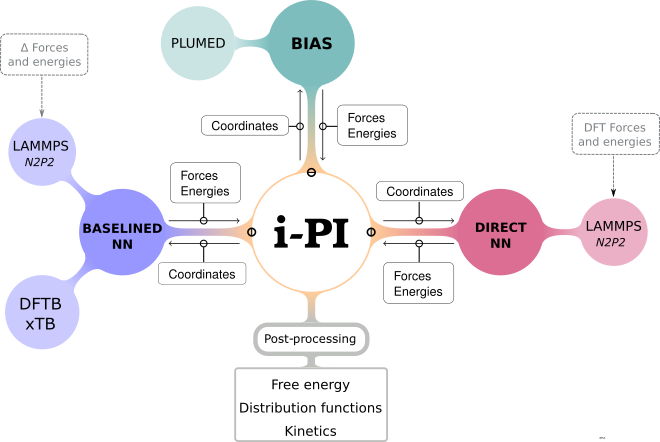
\includegraphics[scale=0.8]{latex_files/diagram_general.png}
    \caption{Scheme of the simulation workflow.}
    \label{fig:workflow}
\end{figure}

\subsection{Launching LAMMPS with the i--PI interface}
\begin{mybox2}{{Input Files, Executables and Scripts}}
\begin{minipage}[c]{0.5\linewidth}
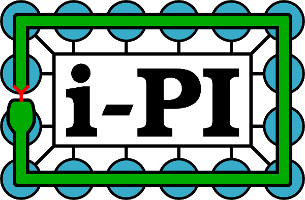
\includegraphics[scale=0.35]{latex_files/ipi-logo-alpha.png}
\end{minipage}
\begin{minipage}[c]{0.5\linewidth}
\begin{itemize}
    \item system.xyz
    \item input.xml
    \item lmp1.in
    \item initial.data
    \item \textcolor{blue}{nnp-parameters} directory
    \item \textcolor{green}{lmp}
\end{itemize}
\end{minipage}
\end{mybox2}

The detailed documentation and tutorials for the codes used here are listed in section \ref{sec:tutorials}. We recommend users get familiar with the inputs and submission commands. Here, we guide to the setting relevant to the application of NNPs. 

In this section, we use the i-PI driver in combination with the n2p2 library, which is part of the LAMMPS code. 

To run MD with the NNP, create a new directory and copy them the following files:
\begin{itemize}
\item input.xml - the input file for i\_PI
\item system.xyz - the xyz coordinates of the initial structure for MD
\item lmp1.in - the input file for LAMMPS
\item initial.data - the same structure as in the system.xyz, but in the LAMMPS format 
\item NNP parameters
\end{itemize}

To extract the parameters of the NNP, create the nnp\_parameters directory and place it in the files obtained during the training, namely: input.data, input.nn, scaling.data and weights.XXX.001000.out. The name of the weight files needs to be changed to format weights.XXX.data. 

Now, let's have look at the content of the different input files. The system.xyz is the starting frame of the MD simulation, which is read by i-PI. The same structure needs to be provided also for the LAMMPS and can be found in the initial.data. The initial data file can be generated by the script get\_lammps.sh.

The input.xml contains the parameters of the molecular dynamics, for example, simulation ensemble, thermostat, temperature, and time step. The energy and forces are computed by an external code, in our case LAMMPS. The connection between the i-PI and LAMMPS is provide via socket interface, specified in the part \textbf{ffsocket}:

\begin{verbatim}
    <ffsocket mode="inet" name="driver-lammps1">
    <address> 192.168.100.1</address>
    <port>8762</port>
    <slots>1</slots>
    <timeout>600</timeout>
    </ffsocket>
\end{verbatim}

In this case, the i-PI and LAMMPs communicate via an inet interface, which is defined by a unique combination of IP address and port. Details of the setting can be found in the i-PI documentation. In general, the i-PI establishes the communication channel using the given address. The external code then connects to this channel to receive and send information. The socket interface prevets the initialization of the external code in every step, which significantly saves computational time. 

The input parameters for the LAMMPS are placed in the lmp1.in file. The NNP specification is described in the pair\_style:

\begin{verbatim}
pair_style nnp dir ${runnerDir} showew no showewsum 1 resetew yes maxew 200000
cflength 1.889726 cfenergy 0.036749

pair_coeff * * ${runnerCutoff}
\end{verbatim}

The pair style informs LAMMPS to use the interaction computed by nnp potentials trained with n2p2. \${runnerDir} variable contains the path to the NNP parameters. The additional parameters control the printing of the extrapolation warning by n2p2. Detailed explanation of possible option is given in the n2p1 tutorial (see section \ref{sec:tutorials}).

The pair\_coeff command contains information on the runner\_cutoff, which is the larger cutoff of the symmetry functions used in the NNP training. It needs to be specified in the LAMMPS units, \textit{i.e.} in Angstrom. 

The last part of the input then specifies the connection to i-PI and the number of steps.

\begin{verbatim}
    fix 1 all ipi 192.168.100.1 8762
\end{verbatim}

To launch the molecular dynamics, initiat the the i-PI by:

\begin{center}
\mybox{\textit{python i-pi input.xml $>>$ ipi.out \&}}
\end{center}

and then launch LAMMPS:

\begin{enumerate}
    \item export LD\_LIBRARY\_PATH=/path/to/n2p2/lib:\$\{LD\_LIBRARY\_PATH\}
    \item lmp -i lmp1.in $>>$ log1.lammps \&
\end{enumerate}

The simulation trajectory will be printed in the simulation.pos\_0.xyz and can be visualized for example by vmd (\url{https://www.ks.uiuc.edu/Research/vmd/}). 

While the NNPs have sufficiently small training errors, the MD will be stable for only a few steps. After that, it will start to produce unphysical geometries and eventually explode. \textbf{The monitoring RMSE itself is therefore not sufficient to estimate the quality of the resulting potentials!} 

To obtain stable and reliable molecular dynamics, the NNP quality needs to be improved significantly. One of the possibilities is to identify the problematic geometries from the molecular dynamics, compute the reference energy and forces and retrain the NNP with the new set of structures. This needs to be often repeated several times until the NNP provides stable and reliable results. The number of needed structures may, however, often reach more than a dozen thousand. Another strategy is to start with the structures generated by a sufficiently good level of theory, for example, the semiempirical method or DFT (\textit{e.g.}, PBE). 

\fancyhead[L]{6. Baselined NNP--MD}
\section{Part 3: From direct to baselined NNP}
%
\subsection{What is baselined NNP?}
In the previous sections, we learned how to generate the NNPs and use them with the i-PI interface. While the NNP trained directly on DFT data provide predictions at impressive speed, they are often difficult to stabilize, especially for complex systems using more than three elements. As demonstrated by the example, stabilization of direct NNPs is not an easy task, even for a small water box. 
A suitable alternative when dealing with large and complex systems is to use so-called baselined NNP.\cite{ramakrishnan2015big} Instead of reproducing directly the DFT data, the baselined NNPs are trained to correct the forces and energy computed at a lower level of theory. The baselined NNPs thus require a lower number of structures and descriptors and are more robust compared to the direct NNP. In the following part, we demonstrate how to train the baselined NNPs adn apply them in the MD.
%
\subsection{Baselined energy and forces}
\begin{mybox2}{{Input Files, Executables and Scripts}}
\begin{minipage}[c]{0.5\linewidth}

\includegraphics[scale=0.15]{latex_files/xtb.png}
\end{minipage}
\begin{minipage}[c]{0.5\linewidth}
\begin{itemize}
    \item input.data
    \item \textcolor{green}{xtb\_ase.py xtb\_io.py}
     
    \item \textcolor{green}{xtb}
\end{itemize}
\end{minipage}
\end{mybox2}
At the beginning, we need to choose a suitable baseline method for the NNP. The baseline can be any computational method which provides reasonable results at computational cost significantly lower the reference. In this tutorial, we use the GFN0-xTB Hamiltonian from the family of xTB methods.\cite{https://doi.org/10.1002/wcms.1493} 

The construction of the baselined NNPs is practically identical to the direct NNP. However, the target properties are not the DFT data but the difference between the DFT and GFN0-xTB results. As a first step, we therefore need to compute the energy and forces for the existing set of structures. For this, we use the xTB v6.2. To automatize the computation, we use ase calculator to prepare the structures and submit the computations. The calculator is available at xtb\_io.py. 

At the beginning, copy the xyz structures used for PBE computations into new folder. Then, use script prepare\_xtb.sh to move every structure to separated dictionary and submit the computations. The example of the submission script is at submit.sh. You will need to modify the path to the xtb and cluster specific settings.

Once the computations are finished, use process\_xtb\_forces.sh to create the forces database and translate\_xtb.f90 to generate new input.data file.

\begin{mybox3}{Output Files}
\begin{itemize}
    \item \textbf{input.data}
\end{itemize}
\end{mybox3}
%
\subsection{The training}
\begin{mybox2}{{Input Files, Executables and Scripts}}
\begin{minipage}[c]{0.5\linewidth}

\includegraphics[scale=0.1]{latex_files/n2p2.png}
\end{minipage}
\begin{minipage}[c]{0.5\linewidth}
\begin{itemize}
    \item new--input.data
    \item input.nn
    \item \textcolor{green}{nnp--scaling}
    \item \textcolor{green}{nnp--train}
\end{itemize}
\end{minipage}
\end{mybox2}

In the next step, create new folder for the training of the NNP, move there input.data and input.nn files and generate the scaling.data file for the new database. Here, we use the same input.nn file as for the direct NNP. However, the best parameters for the baselined NNP might be different. Feel free to experiment with the number of the epoch, size of the training set and test set, ratio of the forces etc.  

In general, the RMSE errors in the training of the baselined NNP will be lower than in the direct case. For the comparison of the baselined and direct NNP, see for example Ref. \citenum{Rossi2020,Juraskova2021}.
\begin{mybox3}{Output Files}
\begin{itemize}
    \item \textbf{learning-curve.out}
    \item \textbf{weights.001.001000.out}
    \item \textbf{weights.008.001000.out}
\end{itemize}
\end{mybox3}
%
\subsection{Baselined--NNP with i--PI}
\begin{mybox2}{{Input Files, Executables and Scripts}}
\begin{minipage}[c]{0.5\linewidth}
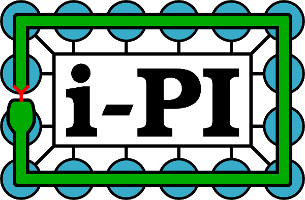
\includegraphics[scale=0.35]{latex_files/ipi-logo-alpha.png}
\end{minipage}
\begin{minipage}[c]{0.5\linewidth}
\begin{itemize}
    \item input.data input.nn scaling.data
    \item weights.001.001000.out weights.008.001000.out
    \item input.xml
    \item initial.data system.xyz
    \item lmp1.in
    \item \textcolor{green}{xtb\_ase.py xtb\_io.py}
\end{itemize}
\end{minipage}
\end{mybox2}

Once the training is finished, you can launch the baselined--NNP MD. The main difference concerning the direct DFT is that apart from the NNP itself, you also need to compute the baseline energy and forces at every step. The input.xml for the i-PI therefore includes computations of forces using additional code, in our case xtb via xtb-ASE calculator. The new lines in the input.xml include two communication channels:

\begin{verbatim}
   <ffsocket mode="inet" name="driver-lammps1">
      <address>192.168.100.117</address>
      <port>8762</port>
      <slots>1</slots>
      <timeout>600</timeout>
    </ffsocket>
    <ffsocket mode='inet' name='driver-xtb'>
     <address>192.168.100.117</address>
     <port>8763</port>
     <slots>1</slots>
     <timeout>600</timeout>
     </ffsocket>

\end{verbatim}

and two force computations:

\begin{verbatim}
    <forces>
      <force forcefield ="driver-lammps1" weight='-1.000'></force>
      <force forcefield ="driver-xtb"></force>
    </forces>
\end{verbatim}

The weight in the first line depends on the definition of your correction in the input.data. In our case, the baselined NNP reproduce xTB - DFT energy and forces.

While the MD with baselined NNP is more stable than with the direct NNP and does not expolde, it still produces unphysical geometries and has large extrapolation earnings (see log1.lammps). The iterative improvement of the NNP is therefore again needed. However, lower number of stuctures will be needed to improve quality of the NNP than in the direct case.

\subsection{Multiple-time-step approach}

In the previous sections, we introduced direct and baselined NNP. While the water box is relatively simple system, we can already see that baselined NNP are more robust in the simulation and are easier to train. However, their application in the molecular dynamics is significantly more expensive than the direct NNP due to cost of the baseline. This limitations become much stronger for complex systems and systems with large number of atoms. 
To decrease the computational cost of the baselined NNP while keep its accuracy, we use so called multiple-time-step approach (MTS).\cite{} 

Here, we use an MTS with a 1-6 scheme, where the energy and forces are computed by a direct NNP using an inner time step of 0.5 fs and corrected by GFN0-xtb and baselined NNP every 3 fs. All the relative keywords are mentioned within the input.xml and the structure of the file does not differ from the previous ones met during the tutorial.

%
\newpage
\fancyhead[L]{7. Supplementary tutorials}
\section{Supplementary tutorials}
\label{sec:tutorials}
\subsection{Tinker(--HP)}
\begin{itemize}
    \item Frédéric CELERSE personnal tutorials (on request): cMD / preparing Tinker xyz files / Umbrella Sampling / Steered Molecular Dynamics / Gaussian accelerated Molecular Dynamics
    \item AMOEBA workshop: \url{https://sites.google.com/site/amoebaworkshop/}
    \item Tinker website: \url{https://dasher.wustl.edu/tinker/}
    \item GitHub (open source code): \url{https://github.com/TinkerTools/tinker}
\end{itemize}
\subsection{n2p2}
\begin{itemize}
    \item GitHub (open source code): \url{https://github.com/CompPhysVienna/n2p2}
    \item Manual: \url{https://compphysvienna.github.io/n2p2/index.html}
\end{itemize}
\subsection{cp2k}
\begin{itemize}
    \item GitHub (open source code): \url{https://github.com/cp2k/cp2k}
    \item cp2k website: \url{https://www.cp2k.org/}
\end{itemize}
\subsection{i--PI}
\begin{itemize}
    \item GitHub (open source code): \url{https://github.com/i-pi/i-pi}
    \item i--PI website: \url{http://ipi-code.org/}
    \item i--PI manual: \url{http://ipi-code.org/assets/pdf/manual.pdf}
\end{itemize}
\subsection{LAMMPS}
\begin{itemize}
    \item GitHub (open source code): \url{https://github.com/lammps/lammps}
    \item LAMMPS website: \url{https://lammps.sandia.gov/}
    \item LAMMPS tutorials: \url{https://icme.hpc.msstate.edu/mediawiki/index.php/LAMMPS_tutorials.html}
\end{itemize}

%\newpage
%\fancyhead[L]{9. Optimal protocol for stable NNP}
%\section{Optimal protocol for stable NNP}
%In this last section, we aim at providing optimal parameters to train a NNP which could be then used for production. Note that the proposed %methods and parameters come from different works available in the literature and modifications might be needed. 
%
%\textbf{SYSTEM CASE}: The user want to model a direct NNP of an azobenzene in order to reproduce an \textit{ab--initio} MD. In this case, the user has to separate two important components:
%\begin{enumerate}
%    \item How he will built his own NNP ?
%    \item How he will train for ?
%\end{enumerate}
%These two features are complementary but have to be treated carefully and separated. Let us see how we suggest to proceed for that !
%\subsection{How to build a good starting NNP ?}
%The complexity as well as the chemical event that any user would like to explore are two crucial parameters to take into account. Here, %there is only 3 different atom types (H,C and N) and the system is made of 24 atoms. In case of the photoswitches, the event could be %decoupled into two main parts:
%\begin{enumerate}
%    \item \textbf{PHOTO}: a photo event comes from by an photo-excitation of the system through any wave length. 
%    \item \textbf{SWITCH}: a switch event is related to the conformation switch of a molecule which is only due to thermal fluctuations.
%\end{enumerate}
%In our case, the photo part needs some external excitations, which is not available in MD--NN based only on the ground state Potential %Energy Surface. Concerning the switch part, we have two available conformations: E and Z. One interesting question should be thus: %\textbf{Which mechanic way should enable the switch of azobenzene from E to Z ?} \\
%To answer to this question, we need thus to prepare the NN according to this specific question. In our case, and according to the %literature, azobenzene could depict two switch mechanisms: the inversion and the rotation. The aim is thus to let the choice of the desired %path within our MD--NN to observe which way is preferred or not. Therefore, the NN has to know the existence of these two ways and %structures taken to build the NN should be part of these pathways. \\
%To generate these structures, you can follow the following instructions:
%\begin{enumerate}
%    \item For each pathway, generate a metadynamics of several ns using a baselined (DFTB+, xTB) using i--Pi coupled to the baselined and %plumed,
%    \item Extract the most relevant structures either manually or by using a clustering method (PCA, TICA, TSNE, ...)
%    \item Only for the most important structures, run a Replica Exchange MD of several ps in order to capture the fluctuation effects from %the temperature. Extract as before the most relevant structures.
%\end{enumerate}
%Once all the structures extracted, we can grab them in order to generate the first dataset which will be used as a starting point for the %procedure. Note that a good compromise for the number of structures to start is localized between 5000 (for simple system) and 10 000 (for %more complex system). 
%%
%\subsection{How to efficiently train a good NNP ?}
%Once the initial dataset was created, the other important part of the work is to design the architecture for future NNP.%
\newpage
\bibliographystyle{achemso}
\bibliography{latex_files/bib}

\end{document}